\section{Desarrollo}
% Metodologia / Desarrollo

La Funcion de Rosenbrock nos presenta una curva similar a un medio circulo, con lo que encontrar el minimo es posible hasta cierto punto, buscarlo
de manera visual, es decir podemos determinar una zona minima. Sin embargo como podemos observar el resultado final %%% Figura Final %%%% 
el minimo se encuentra ligeramente desplazado de donde se esperaria. Esto se debe a la misma funcion que cuenta con una elevacion en la parte inferior
como se puede observar en el zoom de la Figura~\ref{fig: funcion}.

\subsection{Planteamiento del problema y codificación}
Se busca aproximar el mínimo global de la función de Rosenbrock
\[
f(x,y)=100\,{(y-x^2)}^2+{(x-1)}^2,
\]
en un dominio acotado \([x_{\min},x_{\max}]\times[y_{\min},y_{\max}]\). Codificaremos a nuestros individuos, de tal manera que cada solución es un vector \(\mathbf{z}=(x,y)\in\mathbb{R}^2\). Esta codificación evita los costos de decodificación de los esquemas binarios y nos permite aplicar operadores continuos (cruza y mutación).

\subsection{Generar población inicial}
Se genera una población inicial \(\mathcal{P}_0=\{{\mathbf{z}^{(i)}\}}_{i=1}^{N}\) muestreando uniformemente cada dimensión dentro de los límites:
\[
x^{(i)}\sim\mathcal{U}(x_{\min},x_{\max}),\quad
y^{(i)}\sim\mathcal{U}(y_{\min},y_{\max}).
\]
Este muestreo provee una buena diversidad inicial y cobertura del espacio de búsqueda sin sesgos hacia regiones específicas del valle. Al seleccionar una semilla aseguramos la reproducibilidad del experimento.
\begin{figure}[H]
    \centering
    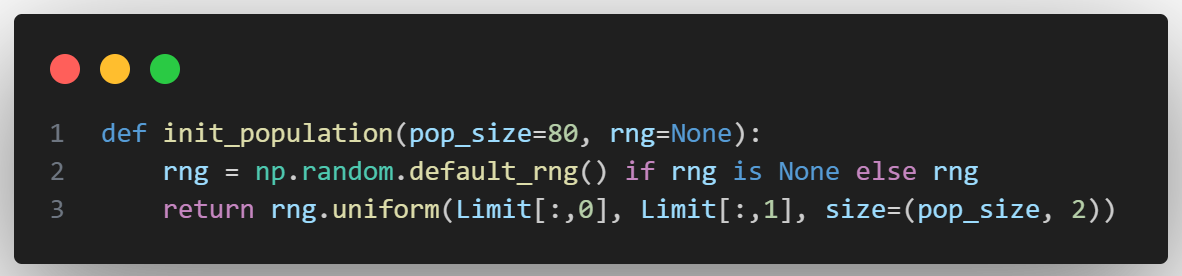
\includegraphics[width=0.7\textwidth]{rsc/img/des/gen_pob.png}
    \caption{Funcion Generadora de Poblacion Inicial}\label{code: gen_pob}
\end{figure}

\subsection{Selección: torneo con \texorpdfstring{$k$}{k} participantes}
Usaremos \textbf{selección por torneo} de tamaño \(k\). Para cada padre, se sortean \(k\) individuos al azar y se elige el de mejor aptitud. De tal manera que:
\begin{enumerate}
    \item Se controla la presión selectiva por medio de \(k\): valores mayores aceleran la explotación; valores menores preservan diversidad.
    \item Es robusta ante reescalamientos de aptitud y evita dependencias de rangos absolutos.
\end{enumerate}
Al implementarlo, la selección se invoca \(N\) veces para formar un multiconjunto de padres \(\mathcal{M}\) con igual tamaño que la población.

\begin{figure}[H]
    \centering
    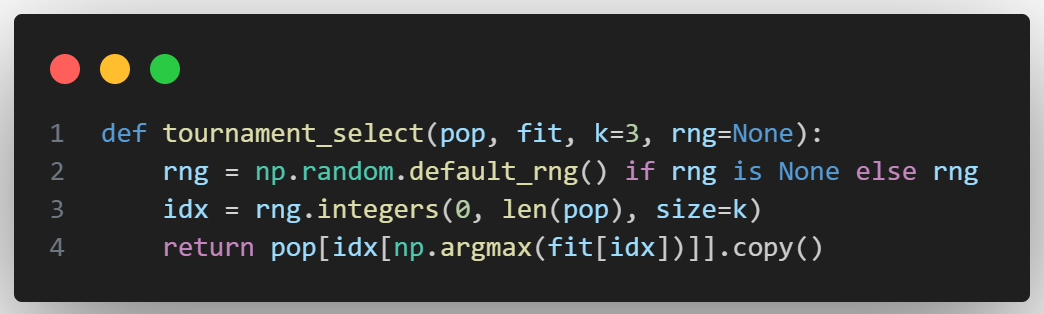
\includegraphics[width=0.7\textwidth]{rsc/img/des/torneo.png}
    \caption{Funcion de Seleccion por Torneo}\label{code: torneo}
\end{figure}

\subsection{Cruza: BLX-\texorpdfstring{$\alpha$}{alpha} (Blend Crossover)}
Para padres \(\mathbf{p}_1\) y \(\mathbf{p}_2\), el operador BLX-\(\alpha\) crea descendientes muestreando, en cada gen \(j\), dentro del intervalo extendido

Se seleccionó BLX-\(\alpha\) es debido a dos razones: (i) extrapolación controlada para cruzar valles curvos sin encasillarse en el segmento entre los padres, e (ii) parametrización simple con \(\alpha\) que equilibra exploración y explotación.

\begin{figure}[H]
    \centering
    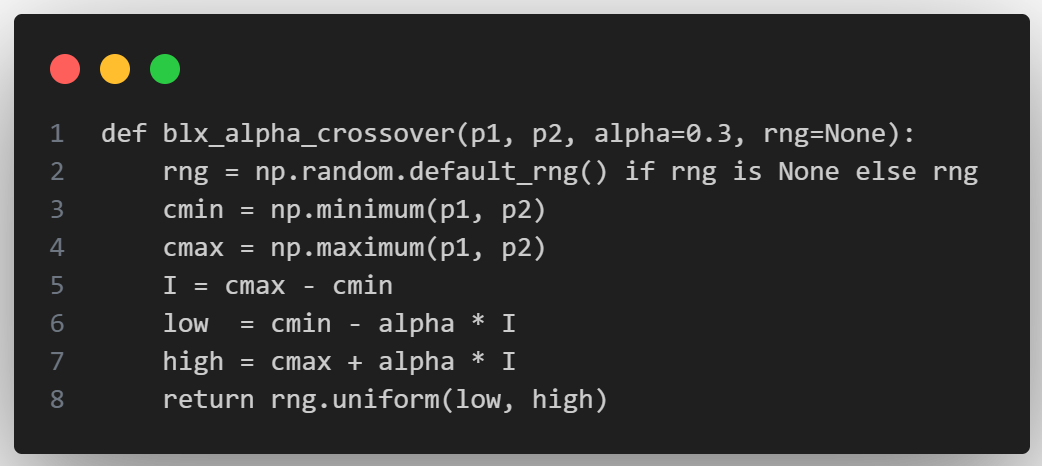
\includegraphics[width=0.7\textwidth]{rsc/img/des/cruza.png}
    \caption{Funcion de Cruza BLX-alpha}\label{code: cruza}
\end{figure}

\subsection{Mutación gaussiana adaptativa}
En cada generación, los individuos pueden modificarse ligeramente aplicando una mutación con una probabilidad \(p\). Esta mutación consiste en agregar un pequeño ruido aleatorio \(\epsilon\) tomado de una distribución normal \(\mathcal{N}(0,\sigma^2)\). El valor de \(\sigma\) controla qué tan grandes son las variaciones y se reduce progresivamente a lo largo de las generaciones.  
De esta forma, al inicio el algoritmo explora con cambios amplios en las soluciones (\(\sigma_{\max}\approx 0.12\)) y, conforme avanza, realiza ajustes más finos (\(\sigma_{\min}\approx 0.01\)) cerca del mínimo.  
Después de aplicar la mutación, los valores que salgan del rango permitido se limitan a los bordes del dominio definido.

\begin{figure}[H]
    \centering
    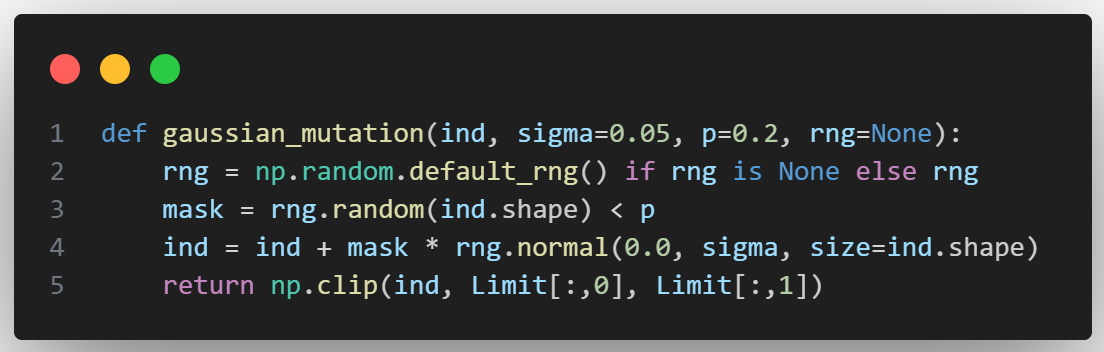
\includegraphics[width=0.7\textwidth]{rsc/img/des/mutacion.png}
    \caption{Funcion de Mutacion Gaussiana Adaptativa}\label{code: mutacion}
\end{figure}

\subsection{Elitismo}
Para asegurar que las mejores soluciones no se pierdan, se conserva un pequeño porcentaje \(\rho\) de los individuos más aptos (alrededor del \(5\%\)) sin modificaciones.  
Estos individuos llamados super individuos se copian directamente a la siguiente generación antes de aplicar los procesos de selección, cruza y mutación.  
El uso del elitismo nos ayuda a mantener la calidad de las soluciones, acelera la convergencia del algoritmo y evita que el azar elimine individuos que ya se encuentran cerca del mínimo global.

\subsection{Estrategias anti-estancamiento}
Para evitar el estancamiento se aplicaron dos estrategias simples que mantienen la diversidad de la población y permiten seguir avanzando hacia mejores soluciones:

\begin{enumerate}
    \item \textbf{Ajuste adaptativo de la mutación}: si el mejor valor no mejora después de varias generaciones, se aumenta ligeramente el valor de \(\sigma\) o la probabilidad de mutación \(p\). Esto introduce más variación en los individuos y ayuda a nuestro algoritmo a explorar nuevas zonas del espacio de búsqueda.
    \item \textbf{Resiembra parcial}: cuando el progreso se detiene por completo, se reemplaza aleatoriamente entre un \(5\%\) y un \(10\%\) de la población, manteniendo siempre a los mejores individuos sin cambios. Esta acción reintroduce diversidad sin afectar el elitismo.
\end{enumerate}

\subsection{Criterios de paro}
Se combinan dos criterios: límite de generaciones \(T\) y un criterio de no-mejora de la mejor aptitud global durante \(T\) generaciones consecutivas. 
Con esto el límite \(T\) limita el costo computacional y la no-mejora detiene la búsqueda cuando el progreso es nulo.

\subsection{Complejidad y parámetros}
En cada generación el algoritmo evalúa a \(N\) individuos y aplica los operadores de selección, cruza y mutación una vez por cada uno, por lo que el costo computacional principal crece de forma lineal con el tamaño de la población, es decir, \(O(N)\). La evaluación de la función objetivo \(f(x,y)\) es muy rápida (\(O(1)\)), por lo que el tiempo total depende principalmente del número de individuos y de generaciones.

Los valores de los parámetros se seleccionaron de manera empírica, buscando un equilibrio entre la exploración del espacio de búsqueda y la velocidad de convergencia:
\begin{itemize}
    \item \textbf{Población} (\(N\)): De 100 a $1,000$ individuos para mantener la diversidad sin aumentar demasiado el costo computacional.
    \item \textbf{Tamaño del torneo} (\(k=3\)): proporciona una presión selectiva moderada, adecuada para la forma estrecha del valle de Rosenbrock.
    \item \textbf{Elitismo} (\(\rho\approx0.05\)): conserva los mejores individuos sin frenar la aparición de nuevas soluciones.
    \item \textbf{Cruza BLX-\(\alpha\)} (\(\alpha\approx0.3\text{--}0.35\)): permite una combinación controlada entre exploración y estabilidad.
    \item \textbf{Mutación} (\(p\approx0.2\text{--}0.25\), \(\sigma_t\) decreciente): asegura una exploración más amplia al inicio y ajustes más finos en las últimas generaciones.
\end{itemize}

\subsection{Visualización y trazabilidad}
Para monitorear el progreso de nuestro algoritmo graficamos nuestra funcion cada cierto numero de generaciones, esto nos permite observar la convergencia de manera clara.
Podemos ver como cada punto (individuo) se va acercando al minimo/maximo global indicado por un rombo rojo en nuestro grafico.

\subsection{Resumen del ciclo genético}
\begin{enumerate}
    \item Evaluar aptitud de \(\mathcal{P}_t\) y extraer élites \(E_t\).
    \item Construir el conjunto de padres con torneo de tamaño \(k\).
    \item Generar hijos mediante BLX-\(\alpha\) por parejas; aplicar \(\mathrm{clip}\).
    \item Mutar con probabilidad \(p\) usando \(\sigma_t\) adaptativa; aplicar \(\mathrm{clip}\).
    \item Insertar élites en la descendencia y formar \(\mathcal{P}_{t+1}\).
    \item Actualizar mejor valor global y aplicar, si corresponde, mecanismos anti-estancamiento.
\end{enumerate}

\subsection{Implementacion}
\subsubsection{minimo}
Poblacion Inicial: 100
Generaciones: 100
Tamaño de torneo: 3

\begin{figure}[H]
    \centering
    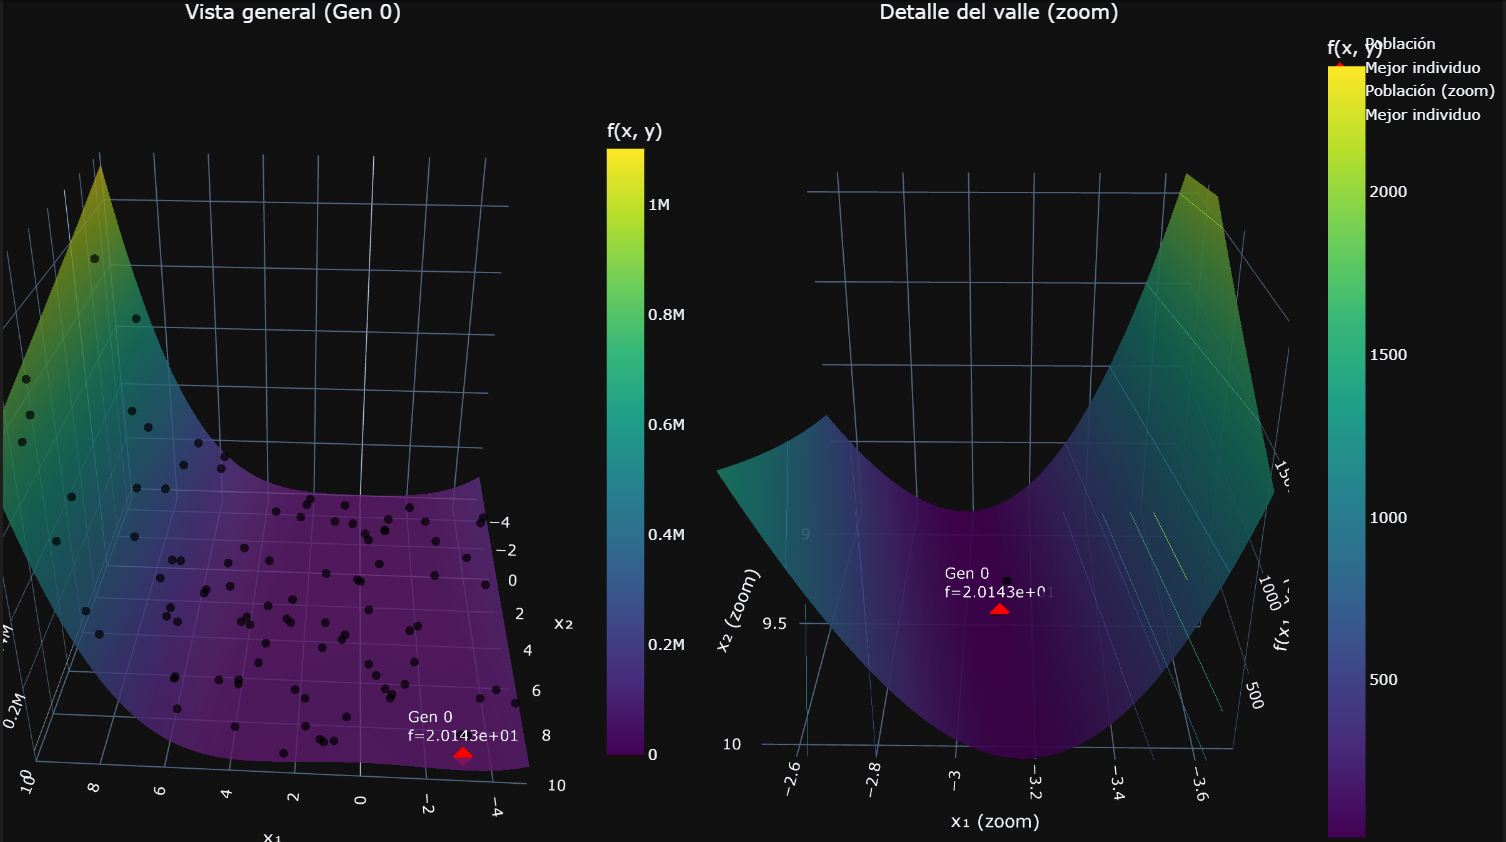
\includegraphics[width=0.9\textwidth]{rsc/img/des/p100_0.png}
    \caption{Funcion de Rosenbrock con poblacion inicial de 100 Gen 0}\label{fig: p100_0}
\end{figure}

\begin{figure}[H]
    \centering
    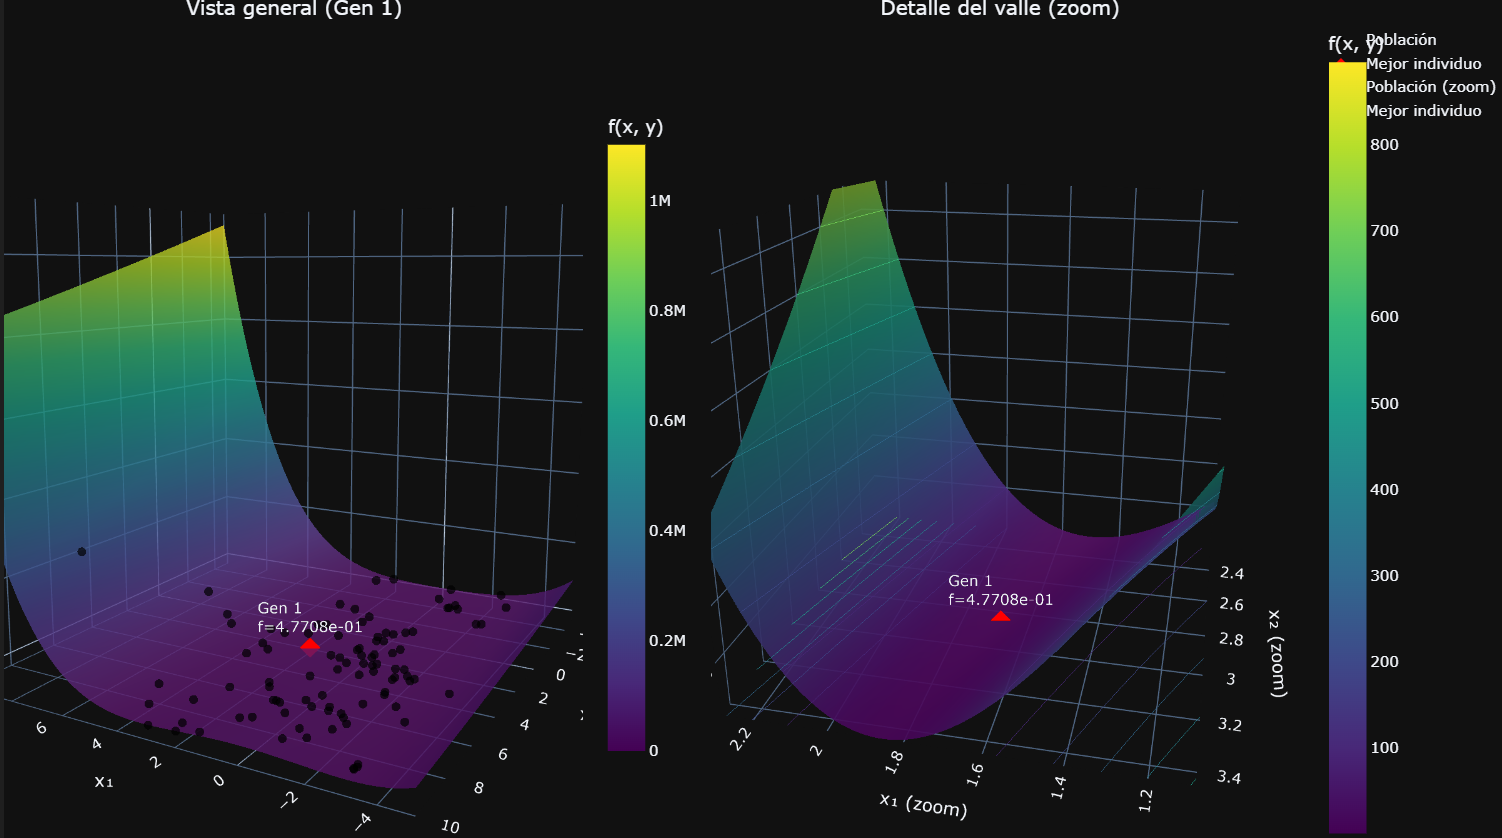
\includegraphics[width=0.9\textwidth]{rsc/img/des/p100_1.png}
    \caption{Funcion de Rosenbrock con poblacion inicial de 100 Gen 1}\label{fig: p100_1}
\end{figure}

\begin{figure}[H]
    \centering
    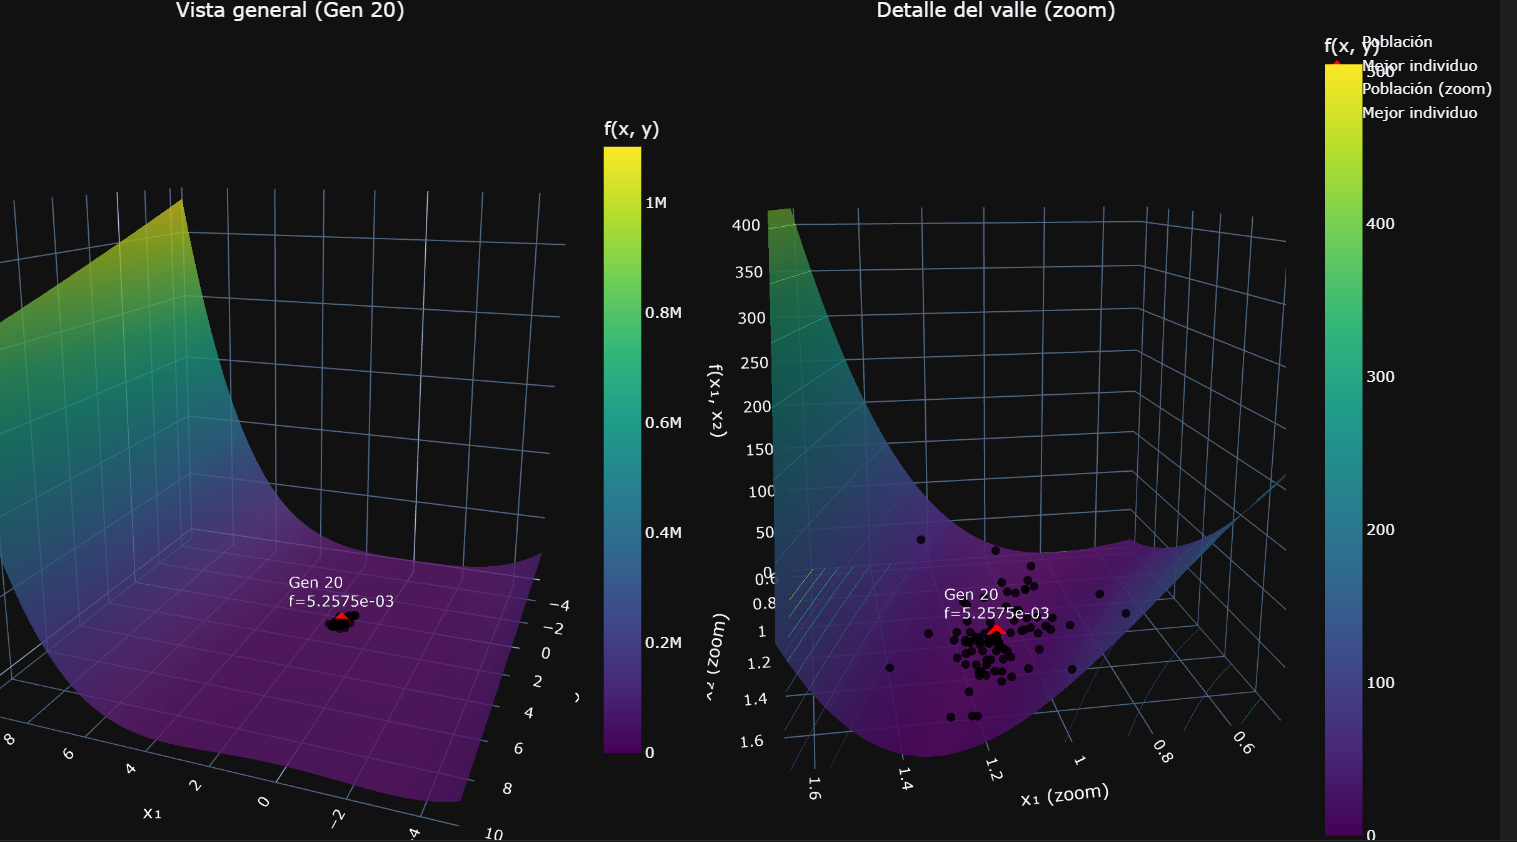
\includegraphics[width=0.9\textwidth]{rsc/img/des/p100_20.png}
    \caption{Funcion de Rosenbrock con poblacion inicial de 100 Gen 20}\label{fig: p100_20}
\end{figure}

\begin{figure}[H]
    \centering
    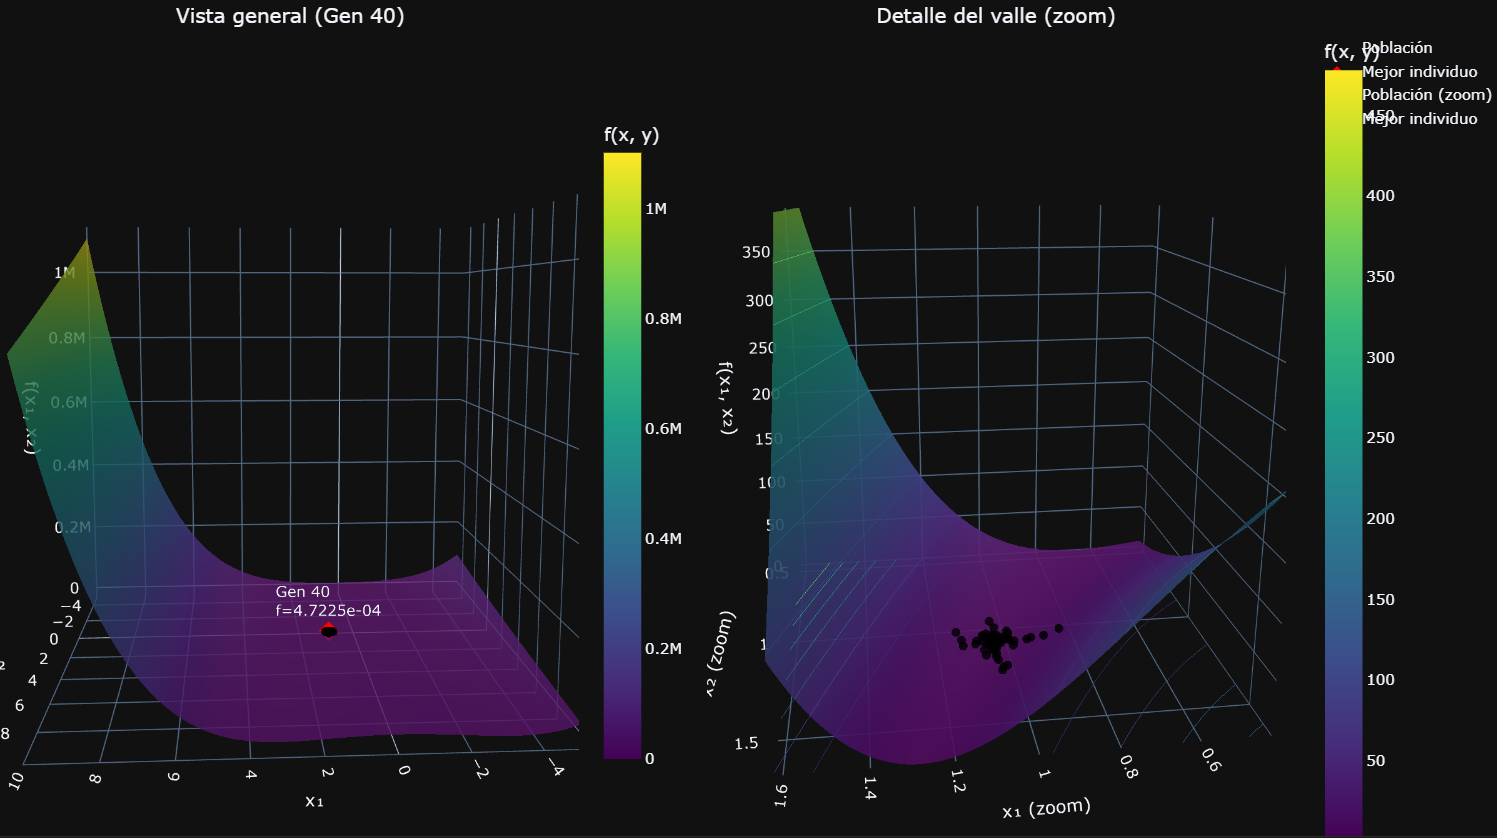
\includegraphics[width=0.9\textwidth]{rsc/img/des/p100_40.png}
    \caption{Funcion de Rosenbrock con poblacion inicial de 100 Gen 40}\label{fig: p100_40}
\end{figure}

\begin{figure}[H]
    \centering
    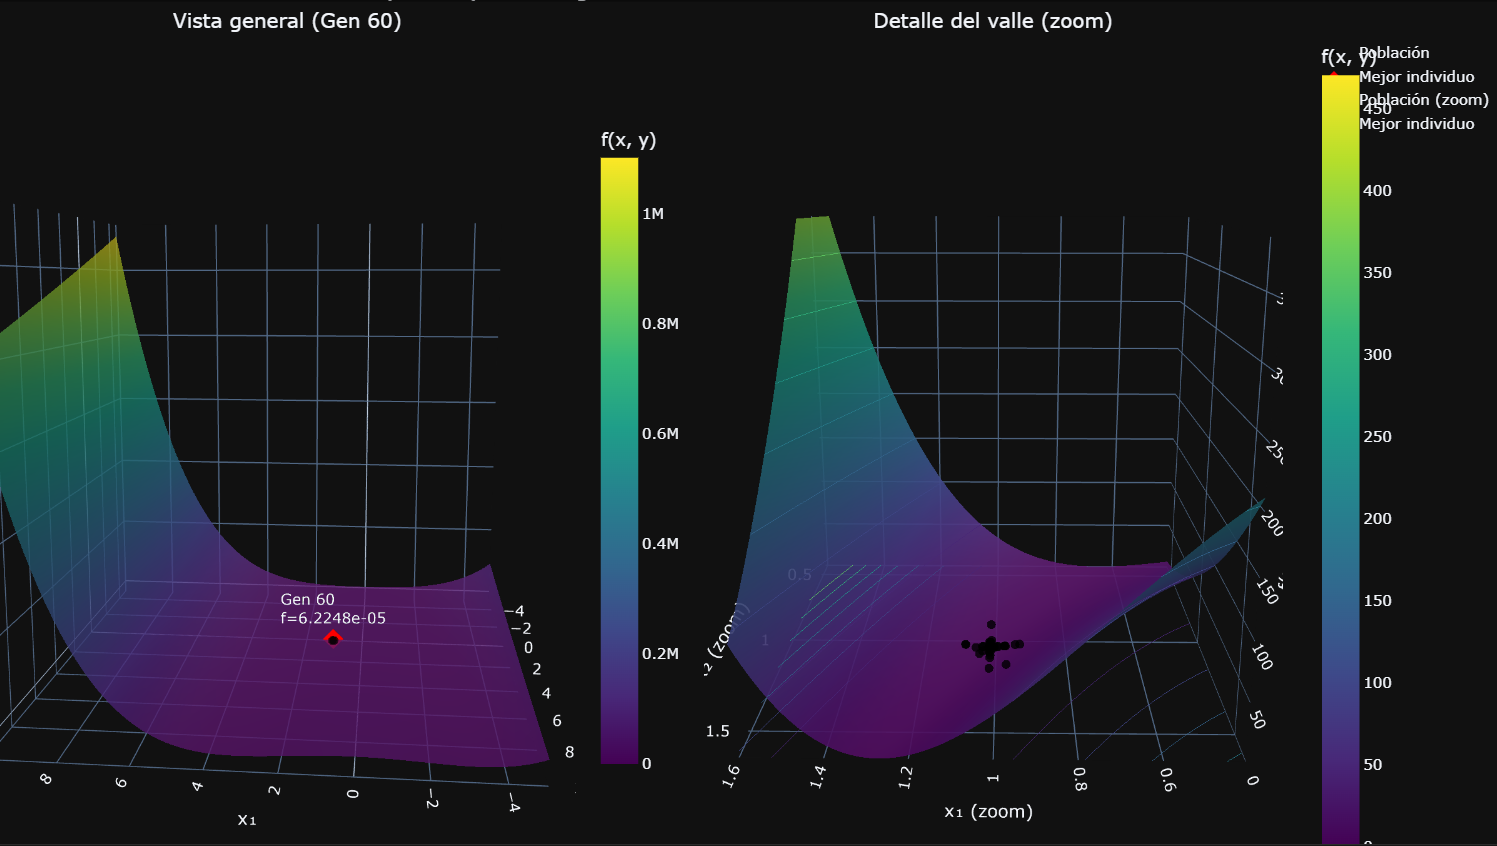
\includegraphics[width=0.9\textwidth]{rsc/img/des/p100_60.png}
    \caption{Funcion de Rosenbrock con poblacion inicial de 100 Gen 60}\label{fig: p100_60}
\end{figure}

Al final nuestro algoritmo se detuvo en la generacion 68 ya que paso 10 generaciones sin cambios.
Obteniendo los siguientes resultados:
\begin{itemize}
    \item Mejor individuo: (x=1.007874, y=1.015761)
    \item Valor de la función en el mejor individuo: $6.224806e-05$
    \item Generación en la que se encontró el mejor individuo: 58
    \item Número total de generaciones ejecutadas: 68
\end{itemize}

\subsubsection{Maximo}
Poblacion Inicial: 100
Generaciones: 100
Tamaño de torneo: 3

\begin{figure}[H]
    \centering
    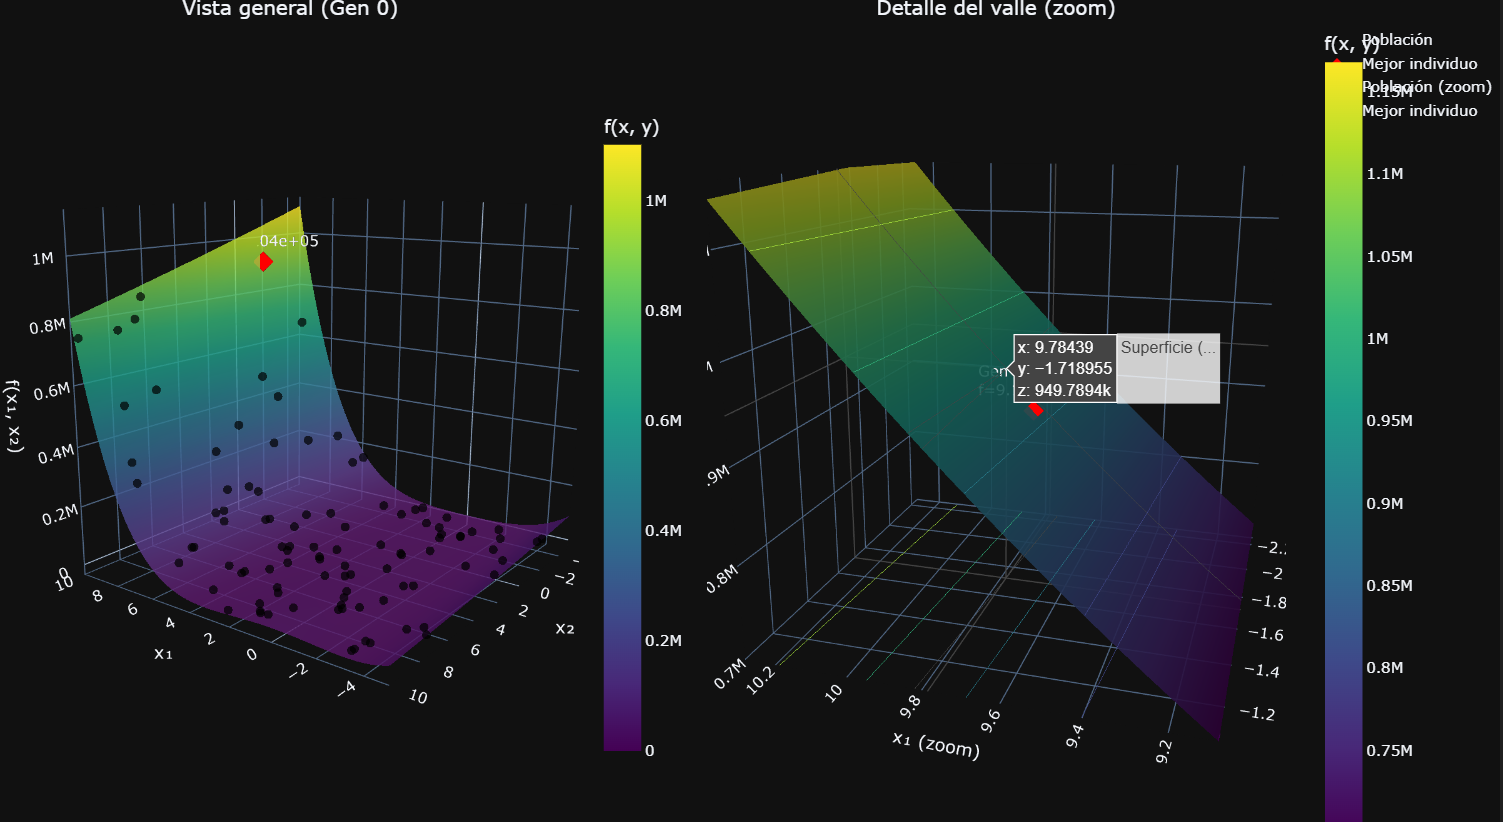
\includegraphics[width=0.9\textwidth]{rsc/img/des/p100_0_max.png}
    \caption{Funcion de Rosenbrock con poblacion inicial de 100 Gen 0}\label{fig: p100_max_0}
\end{figure}

\begin{figure}[H]
    \centering
    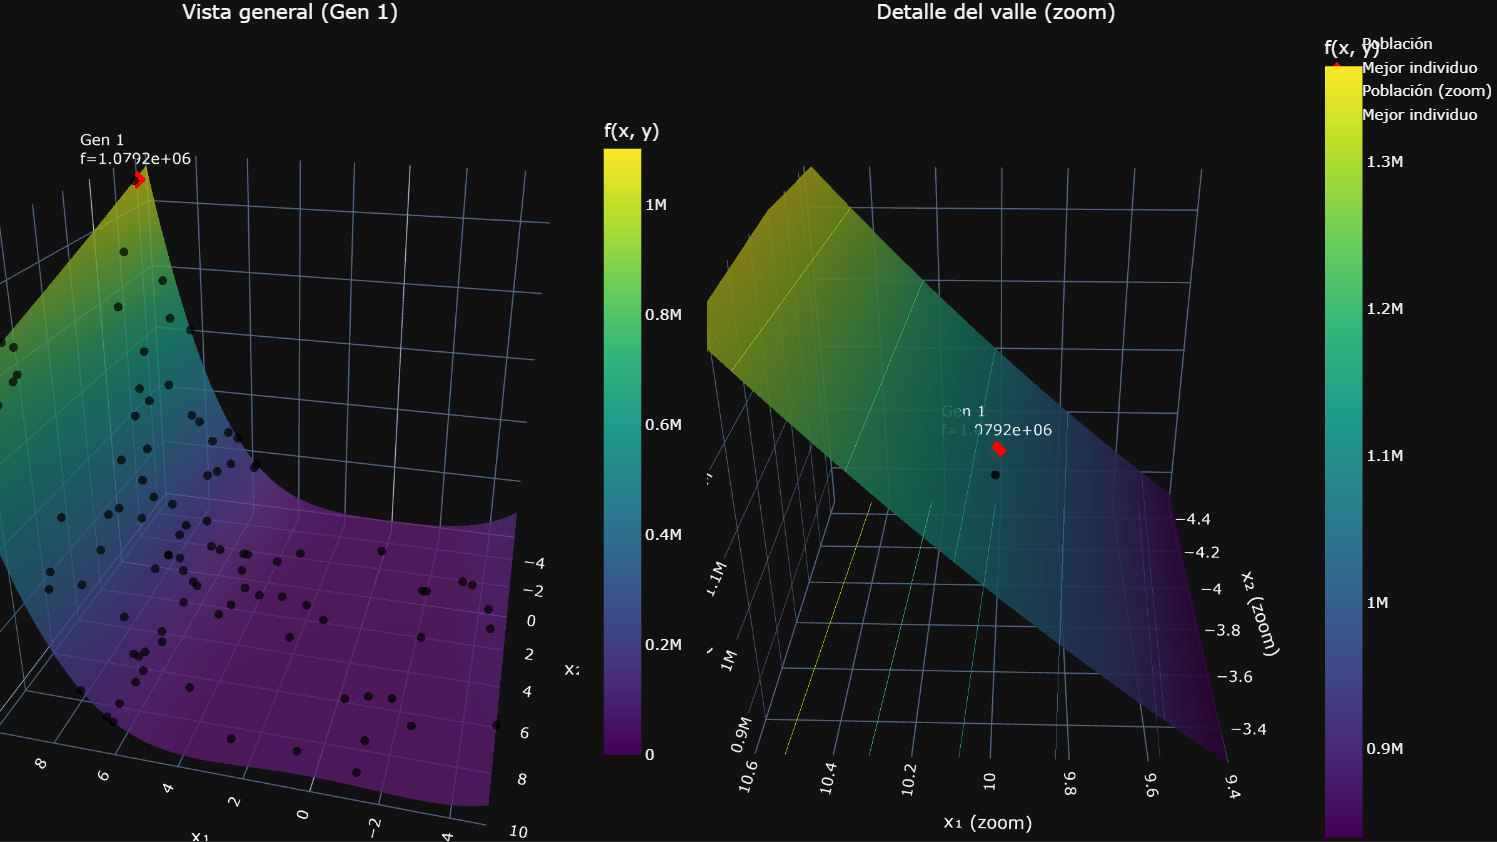
\includegraphics[width=0.9\textwidth]{rsc/img/des/p100_1_max.png}
    \caption{Funcion de Rosenbrock con poblacion inicial de 100 Gen 1}\label{fig: p100_max_1}
\end{figure}

\begin{figure}[H]
    \centering
    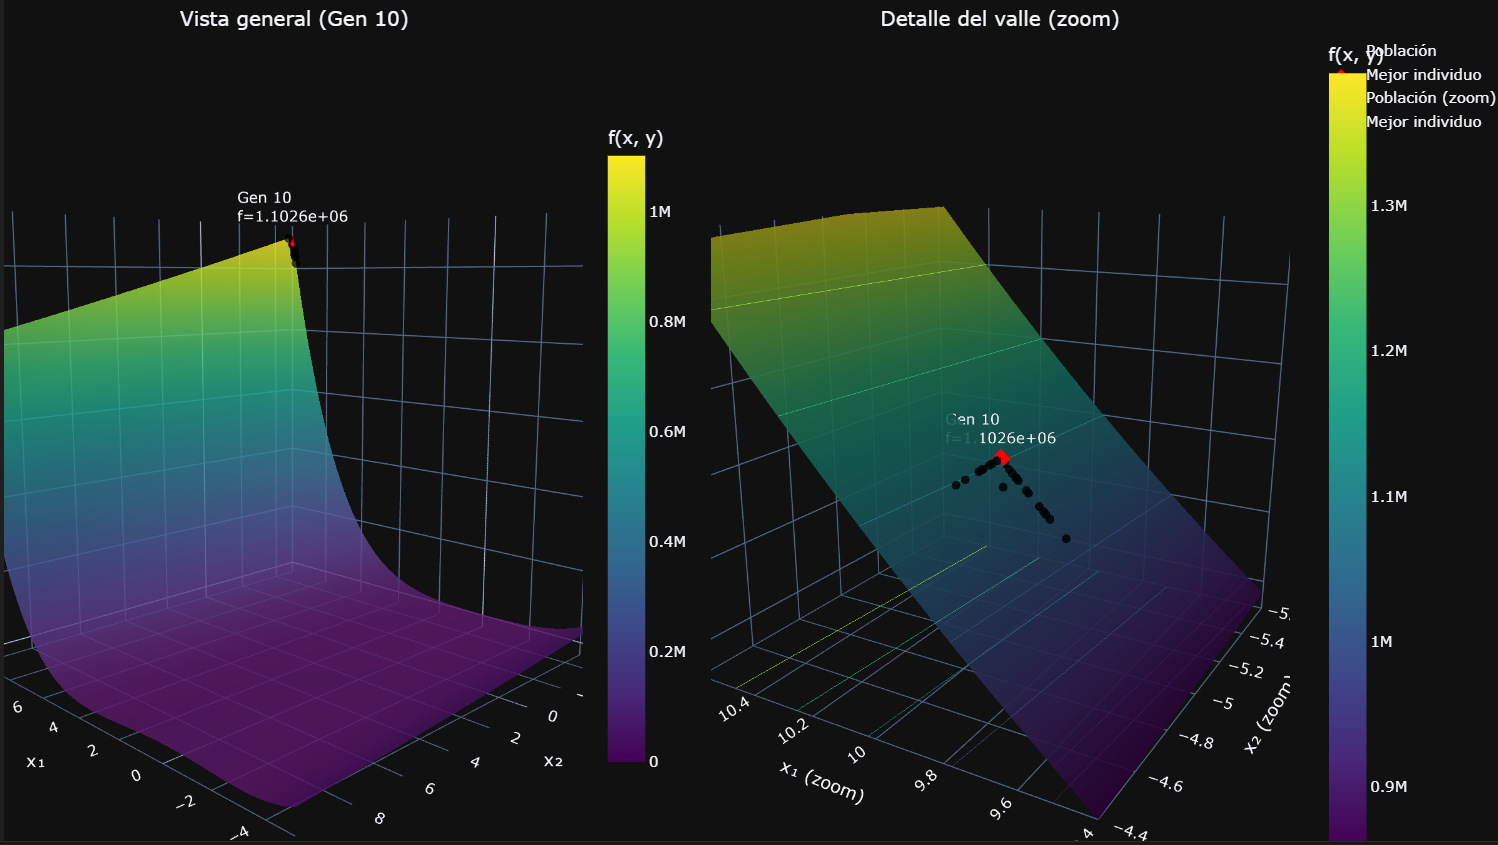
\includegraphics[width=0.9\textwidth]{rsc/img/des/p100_10_max.png}
    \caption{Funcion de Rosenbrock con poblacion inicial de 100 Gen 10}\label{fig: p100_max_10}
\end{figure}
Al final nuestro algoritmo se detuvo en la generacion 12 ya que paso 10 generaciones sin cambios.
Obteniendo los siguientes resultados:
\begin{itemize}
    \item Mejor individuo: (x=10.000000, y=-5.000000)
    \item Valor de la función en el mejor individuo: $1.102581e+06$
    \item Generación en la que se encontró el mejor individuo: 2
    \item Número total de generaciones ejecutadas: 12
\end{itemize}